%!TEX root = master.tex

\section{\$ java -is-dynamic}

\begin{frame}
  \frametitle{\$ java -is-dynamic}

  But can Java be considered a dynamic language ? 
  \vspace{0.4cm}
  \begin{center}
  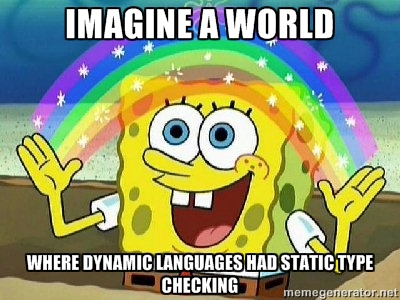
\includegraphics[width=0.7\textwidth]{fig/dynlang}    
  \end{center}
\end{frame}

\begin{frame}
  \frametitle{\$ java -is-dynamic}
  \center

  "The term dynamic programming language describes a class of programming languages that share a number of common runtime characteristics that are available in static languages only during compilation, if at all.[…]” 

  \vspace{0.3cm}

  “[…]These behaviors can include the ability to extend the currently running program […] even by modifying the internals of the language itself, all during program execution. While these behaviors can be emulated in almost any language […] such behaviors are integral, built-in characteristics of dynamic languages.”
  \vspace{0.3cm}

T. Mikkonen and A. Taivalsaari,
“Using JavaScript as a real programming language” 2007.

\end{frame}

\begin{frame}
  \frametitle{\$ java -is-dynamic}
  \center
  So, can Java \frqq extend a currently running program\flqq, maybe \frqq even by modifying the internals of the language itself, all during program execution\flqq ?

  \vspace{0.25cm}
  \begin{itemize}
    \item Java reflection can modify certain aspects during runtime
    \vspace{0.4cm} 
    \item The Java class loader can load source code during runtime
    \vspace{0.4cm}      
    \item Javassist (Library) can create/modify Java classes during runtime
    \vspace{0.4cm}    
    \item But: It's a workaround (a hack)
    \vspace{0.4cm}
    \item So it's not an \frqq integral, built-in characteristic\flqq of Java
  \end{itemize}
\end{frame}

\begin{frame}
  \frametitle{\$ java -is-dynamic}

  Dynamic check list
  \vspace{0.25cm}
  \begin{itemize}
    \item Interactive (JavaREPL, wait for demo)
    \vspace{0.4cm} 
    \item Everything is an object (almost)
    \vspace{0.4cm}      
    \item Dynamic Typing (Simulated by using Object, wait for demo)
    \vspace{0.4cm}    
    \item Most things changeable at run-time (Well, it's hacky)
    \vspace{0.4cm}
    \item Reflection (Yes!)
    \vspace{0.4cm}
    \item Late-Bound Everything (Simulated by using Object, wait for demo)
    \vspace{0.4cm}
    \item Garbage Collected (Yes!)
    \vspace{0.4cm}
    \item Interpreted (Yes!)
  \end{itemize}
\end{frame}

\begin{frame}
  \frametitle{\$ java -conclusion}

  \vspace{0.25cm}
  \begin{itemize}
    \item Java is almost a dynamic language
    \vspace{0.4cm} 
    \item It can be stretched alot, but it hurts
    \vspace{0.4cm}      
    \item Not meant to be used this way
    \vspace{0.4cm}    
    \item Not necessarily a bad thing
    \vspace{0.4cm}
    \item Java sits between Python and C++
    \vspace{0.4cm}
    \item However, a lot of dynamic languages compile down to Java byte code!
    \vspace{0.4cm}
    \item Clojure, Jython, JRuby, and A LOT of others
  \end{itemize}
\end{frame}